\documentclass{article}

\usepackage{amsmath}
\usepackage{amssymb}
\usepackage[spanish]{babel}
\usepackage[margin=1.5in]{geometry}
\usepackage{graphicx}
\usepackage{tcolorbox}
\usepackage[utf8]{inputenc}
\usepackage{hyperref}
\hypersetup{
    colorlinks,
    citecolor=black,
    filecolor=black,
    linkcolor=black,
    urlcolor=black,
}

\tcbuselibrary{theorems}

\renewcommand{\Bbb}{\mathbb}

\title{Apuntes de EDO de Análisis Matemático II A (63.01) \\ Cátedra Acero \\ 1° C 2004}
\author{Darío Eduardo Ramos}

\begin{document}
\maketitle

\tableofcontents{}
\newpage

\section{Definiciones previas}

Una función escalar es diferenciable si y sólo si se puede escribir lo siguiente:

\begin{equation}
f(x+h) - f(x) = \underbrace{f'(x) h}_{\text{diferencial total}} + \underbrace{ \mu(h) h }_{\text{infinitésimo}}
\end{equation}

En el lado derecho de esta igualdad, el primer sumando es el \textbf{diferencial total de la función}, y el segundo es un infinitésimo: tiende a cero cuando h tiende a cero.

Propiedades:

\begin{subequations}
\begin{align}
d k & = 0 \\
d(k f) & = k \mathop{df} \\
d(f \pm g) & = \mathop{df} \pm \mathop{dg} \\
d(f g), d( f / g ) & = \textbf{igual que derivada} \\
\mathop{dy} & = f'(x) h \wedge h = \mathop{dx} \Longrightarrow y' = \frac{\mathop{dy}}{\mathop{dx}} = f'(x)
\end{align}
\end{subequations}

Esta última se conoce como la notación de Leibnitz.

Una ecuación diferencial, o ED, es una ecuación donde las incógnitas son funciones; toda ED relaciona una función a determinar, su(s) variable(s) independiente(s), y las derivadas y/o diferenciales de la función. Las EDs pueden ser:

\begin{itemize}
\item Ordinarias: La función incógnita tiene una sola variable independiente.
\item En derivadas parciales: La función incógnita tiene más de una variable independiente.
\end{itemize}

\subsection{Orden de una ED}

El orden de una ED está dado por la derivada de mayor orden de la función incógnita.

\subsection{Expresión general para EDOs (1 variable independiente)}

Expresión general orden 1:

\begin{equation}
F(x, y, y') = 0
\end{equation}

Normalizada orden 1:

\begin{equation}
y' = g(x, y)
\end{equation}

Expresión general para orden N:

\begin{equation}
F(x, y, y', y'', \ldots, y^{(n)}) = 0
\end{equation}

Se dice que $x, y, y', \ldots, y^{(n)}$ son las variables de la ED $F$. La ecuación general ordinaria de orden $n$ tiene entonces $(n+2)$ variables: las $n$ derivadas, $x$ e $y$.

\subsection{Grado de una ED}

Aquellas ED que pueden expresarse como polinomios respecto al orden de las derivadas, y donde además los coeficientes que multiplican a las derivadas son constantes o funciones de $x$, tienen \textbf{grado}. El mismo corresponde al exponente al que está elevada la derivada de mayor orden.

Si algún coeficiente depende de $y$, la ED no tiene grado.

\subsection{Soluciones de una ED}

Sea $y = g(x)$ una función definida en un intervalo $I$, con $n$ derivadas continuas en dicho intervalo. Si al reemplazar $y$ en una ED, la misma se reduce a una identidad, se dice que $y = g(x)$ es solución de la ED en $I$. En tal caso, $I$ es denominado intervalo de solidez, intervalo de existencia, o dominio de la solución.

Tipos de solución:

\begin{itemize}
\item \textbf{Solución general (SG)}: La SG de una ED de orden $n$ es una relación funcional entre sus variables 
que contiene $n$ constantes arbitrarias linealmente independientes.

\item \textbf{Solución particular (SP)}: Se obtiene a partir de la SG al darle valores concretos a sus constantes; usualmente, ello requiere $n$ valores iniciales o condiciones de contorno de la función incógnita y sus derivadas.

\item \textbf{Solución singular (SS)}: Una función es SS de una ED cuando la reduce a una identidad, pero no puede obtenerse a partir de una SG. No toda ED tiene SS.
\end{itemize}

\section{Conceptos generales}

\subsection{Teorema Fundamental del Cálculo}

El TFC plantea que dos funciones $f$ y $g$, definidas en un mismo dominio, difieren en una constante $\Leftrightarrow$ sus derivadas son iguales. Esto implica que al resolver una integral, se obtiene siempre una familia de primitivas:

\begin{equation}
\int f(x) dx = F(x) + C \Leftrightarrow F'(x) = f(x)
\end{equation}

\subsection{Isoclinas y conjuntos de nivel}

Dada una familia de curvas, las isoclinas de nivel $k$ son las curvas que unen los segmentos tangentes de pendiente $k$. Simbólicamente:

\begin{equation}
y' = F(x,y) \Rightarrow I_k = \{(x,y) \in Dom(F) / F(x,y) = k\}
\end{equation}

Las isoclinas son las curvas de nivel de la función derivada.

\begin{figure}[ht]
\caption{Isoclinas}
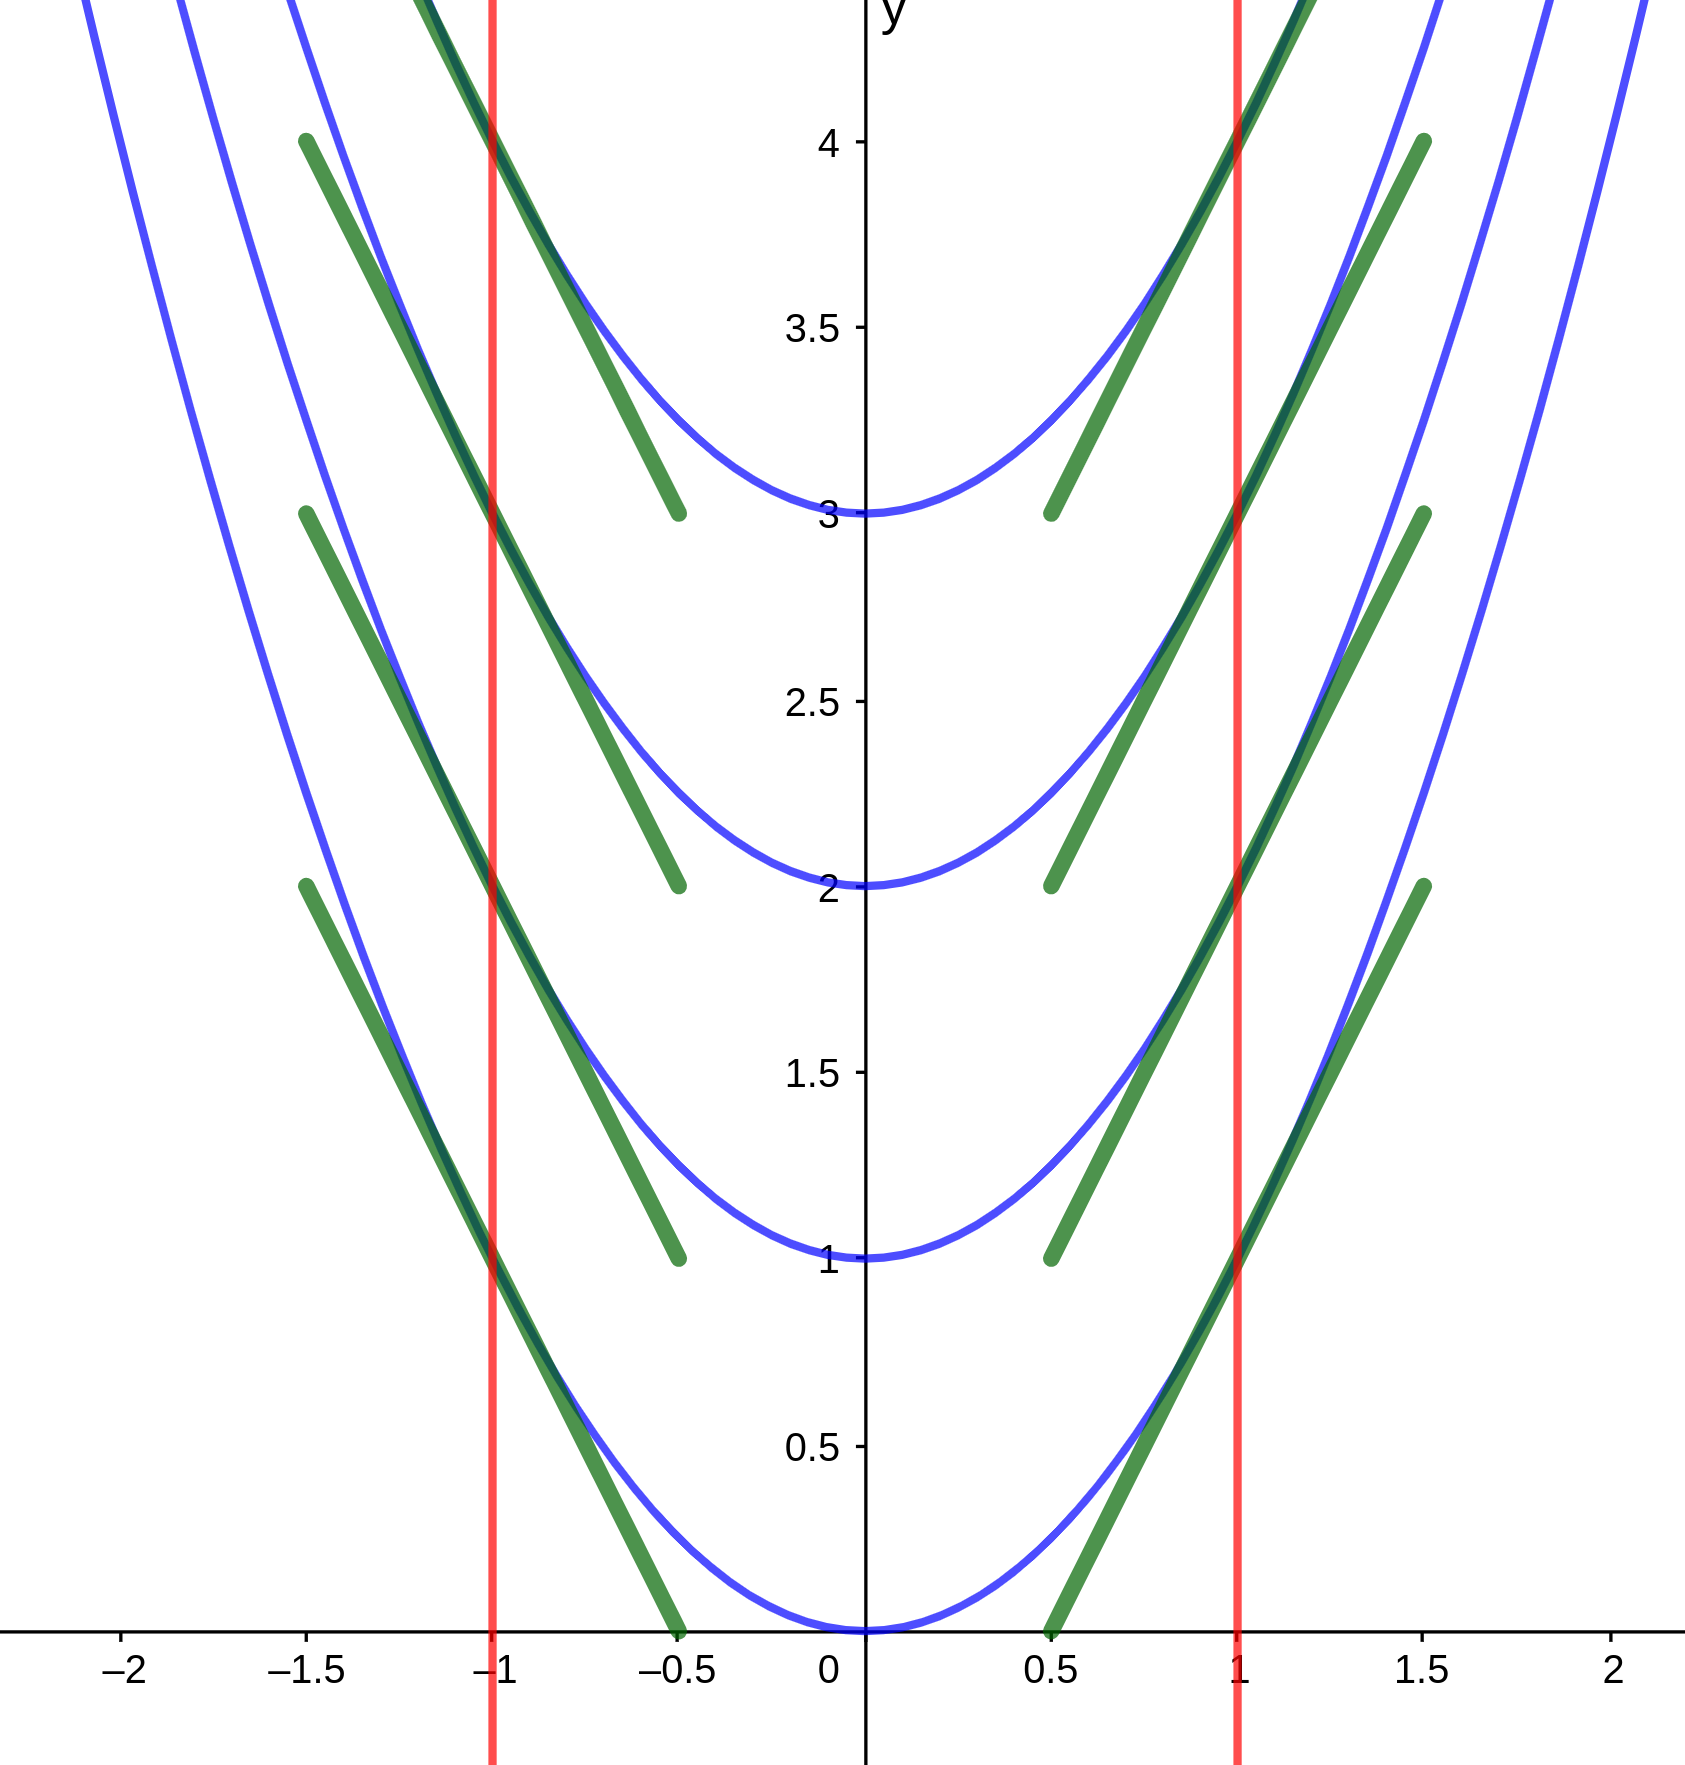
\includegraphics[scale=1]{img/edo/isoclinas.png} 
\centering
\label{fig:isoclinas}
\end{figure}

Por ejemplo, dada una familia de curvas parabólicas (azul), obsérvese la figura ~\ref{fig:isoclinas} en los puntos donde la tangente (verde) es igual, se unen los puntos obteniendo una recta (rojo). Esa es la isoclina para ese valor en particular. Nótese que hay tantas curvas isoclinas como valores tome la derivada; en el gráfico se muestra una sola.

\subsection{Formando EDOs a partir de una familia de curvas}

Sea $F(x, y, C_1, C_2, \ldots, C_n)$ una familia de curvas. Habiendo $n$ constantes independientes entre sí, al derivar $F$ $n$ veces consecutivas surge un sistema de $n$ ecuaciones a partir del cual se podrá obtener una ecuación diferencial. Por ejemplo:

\begin{equation}
y = C_1 \cos(x) + C_2 \sin(x)
\end{equation}

Hay dos constantes independientes; por lo tanto, derivando dos veces respecto a $x$:

\begin{subequations}
\begin{align}
y' = -C_1 \sin(x) + C_2 \cos(x) \\
y'' = -C_1 \cos(x) - C_2 \sin(x)
\end{align}
\end{subequations}

Sumando las expresiones para $y$ e $y''$ miembro a miembro, se obtiene la ED $y + y'' = 0$, que es de segundo grado, lo cual es consistente con el hecho de que haya dos constantes independientes en la definición de la familia de curvas.

A veces, las constantes no son independientes entre sí, aunque lo parezcan. Por ejemplo:

\begin{equation}
y = A + \ln \left( \frac{B}{x} \right) \Rightarrow y = \ln C + \ln \left( \frac{B}{x} \right) = \ln \left( \frac{C B}{x} \right) = \ln \left( \frac{K}{x} \right)
\end{equation}

Así, lo que parecía de segundo orden, es realmente de primer orden. Derivar una vez alcanza para obtener la ED:

\begin{equation}
y' = \frac{1}{\frac{K}{x}} -\frac{K}{x^2} \Rightarrow y' = \frac{-1}{x}
\end{equation}

Si una familia de curvas es solución pero está expresada implícitamente (por ejemplo, círculos), puede que haya que determinar su dominio de validez.

\section{Clases de ED con resolución analítica directa}

\subsection{Variables separables}

Una ED es de VS si y sólo si puede expresarse como el producto entre una función de $x$ y una función de $y$. Formalmente:

\begin{equation}
\text{Una E.D. es de VS} \Leftrightarrow y' = h(x) g(y)
\end{equation}

Resolución: Se asocia $g(y)$ con $dy$, $h(x)$ con $d(x)$ y se integra m. a m. Ejemplo:

\begin{equation}
(1+x) dy - y dx = 0 \Leftrightarrow (1+x) dy = y dx \Leftrightarrow \int \frac{dy}{y} = \int \frac{dx}{1+x}
\end{equation}

Antes de integrar m. a m., tener en cuenta que los ceros de los denominadores pueden ser soluciones singulares (SS), en tanto no se puedan obtener de la solución general obtenida al integrar:

\begin{equation}
\ln |y| = \ln |x + 1| + C \Leftrightarrow |y| = e^{\ln |x+1| + C } \Leftrightarrow |y| = \underbrace{e^C}_{k} e^{ln |x+1|} \Leftrightarrow \underbrace{y = A |x+1|}_{SG}
\end{equation}

En el último paso, se elimina el módulo de $y$ reemplazando la constante positiva $k$ (siempre es positiva por ser una potencia) por una constante $A$ que puede tomar cualquier signo.

Considerando los ceros de los denominadores, $y = 0$ es una SP asociada a $A = 0$. Por otro lado, $x = -1$ es efectivamente una SS.

\subsection{Lineales}

Las ED lineales son aquellas de la forma $y' + s(x) y = T(x)$, con $y$ definida sobre un intervalo donde $s$ y $T$ sean continuas. Hay varios métodos de resolución, entre ellos:

\subsubsection{Variación de parámetros}

Se considera la ecuación homogénea asociada, $y' + s(x) y = T(x)$. Puede demostrarse que $SG(x) = y_H + y_P$, donde $y_H$ es la solución de la ecuación homogénea, e $y_P$ es una solución particular de la ED original.

Dado que la ecuación homogénea es de variables separables, puede calcularse $y_H$ con el método ya visto.

Para obtener $y_P$, si se obtuvo $y_H = C_1 y_1(x)$, puede demostrarse que $y_P(x) = L(x) y_1(x)$ es una SP de la ED original. Reemplazando esa expresión de $y_P$ en la ED, queda una ecuación de variables separables, a partir de la cual puede obtenerse la incógnita $L(x)$ y así obtener la solución final sumando $y_H$ e $y_P$.

Este método (aplicando ciertas generalizaciones) puede usarse para ecuaciones de mayor orden; en todo caso, como suele ser el caso, no sirve para todos los casos, y por eso se ven otros métodos.

\subsubsection{Lagrange}

Dada la ED lineal $y' + s(x) y = T(x)$, se propone como solución el producto $y = u(x) v(x)$. Reemplazando esto en la ED, resulta:

\begin{equation}
\underbrace{u'v + uv'}_{y'} + s(x) \underbrace{uv}_{y} = T(x)
\end{equation}

Sacando factor común $v$ (también se puede hacer con $u$):

\begin{equation}
v (u' + u s(x)) + uv' = T(x)
\end{equation}

Exigiendo que el paréntesis sea nulo, resulta una ecuación en variables separables a partir de la cual se puede obtener $u(x)$.

Tomando una SP de u, se reemplaza y queda $uv' = s(x)$, que de nuevo es de variables separables, y determina a $v(x)$.

Conocidos $u(x)$ e $y(x)$, se conoce la SG $y = u(x) v(x)$.

\subsection{Reducción de orden}

De forma general, la reducción de orden es un método que consiste en plantear una sustitución que reduzca el orden de la ED, idealmente a orden 1. Por ejemplo, dada la EDO:

\begin{equation}
xy''' - y'' = 3x
\end{equation}

Una sustitución conveniente es $\rho = y''$, que conduce a una ecuación lineal:

\begin{equation}
x \rho' - \rho = 3x \Rightarrow \rho' - \frac{1}{x} \rho = 3
\end{equation}

Resolviendo con el método de Lagrange, se plantea: $\rho = u v$:

\begin{equation}
\rho = u v \Rightarrow uv' + uv' - \frac{1}{x} uv = 3 \Rightarrow v \underbrace{ \left(u' - \frac{1}{x} u \right) }_{0} + uv' = 3
\end{equation}

Resolviendo el paréntesis para hallar $u$, es de variables separables:

\begin{equation}
u' - \frac{1}{x} u = 0 \Rightarrow \frac{du}{dx} = \frac{1}{x} u \Rightarrow \int \frac{1}{u} du = \int \frac{1}{x} dx \Rightarrow \ln |u| = \ln |x| + C_1 \Rightarrow u = k x
\end{equation}

En la ecuación de $u$, tomando como solución particular $u = x$ (obtenida con $k=1$), se calcula $v$ usando el segundo sumando en la ecuación de Lagrange:

\begin{equation}
u v' = 3 \wedge u = x \Rightarrow x v' = 3 \Rightarrow x \frac{dv}{dx} = 3 \Rightarrow \int dv = \int \frac{3}{x} dx \Rightarrow v = 3 \ln |x| + C_2
\end{equation}

Conocidos $u$ y $v$, queda determinado $\rho$:

\begin{equation}
\rho = u v \Rightarrow \rho = x (3 \ln |x| + C_2)
\end{equation}

Para obtener $y$, hay que integrar $\rho$ dos veces:

\begin{equation}
y'' = \rho \Rightarrow \frac{d^2y}{dx^2} = x (3 \ln |x| + C_2) \Rightarrow \int \frac{d^2y}{dx} = \int x (3 \ln |x| + C_2) dx
\end{equation}

Distribuyendo:

\begin{equation}
\frac{dy}{dx} = 3 \int x \ln |x| dx + C_2 \int x dx
\end{equation}

Para resolver la primera integral, dado que hay un módulo, hay que considerar dos casos: $x>0$ y $x <0$ ($x=0$ queda fuera porque es una singularidad de la función $\ln$).

\subsubsection{\texorpdfstring{$x > 0$}{x > 0}}

Si $x > 0$, simplemente se va el módulo del logaritmo:

\begin{equation}
z_1 = 3 \int x \ln(x) dx
\end{equation}

Por tabla, $\int x \ln(x) dx = -\frac{1}{4} x^2 + \frac{1}{2} x^2 \ln(x) + C$. Aplicando:

\begin{equation}
z_1 = 3  \left( -\frac{1}{4} x^2 + \frac{1}{2} x^2 \ln (x) + K_1 \right)
\end{equation}

\subsubsection{\texorpdfstring{$x < 0$}{x < 0}}

Si $x < 0$, hay que negar x en el módulo:

\begin{equation}
z_2 = 3 \int x ln(-x) dx 
\end{equation}

Se propone el cambio de variable $\alpha = -x \Rightarrow d\alpha = -dx$:

\begin{equation}
z_2 = 3 \int (-\alpha) \ln(\alpha) (-d\alpha) \Rightarrow z_2 = 3 \int \alpha \ln(\alpha) d\alpha
\end{equation}

Es la misma integral, pero evaluada en $-x$:

\begin{equation}
z_2 = 3 \left( -\frac{1}{4} x^2 + \frac{1}{2} x^2 \ln(-x) + K_2 \right)
\end{equation}

Volviendo a la EDO, es evidente que tiene al menos dos soluciones generales diferentes. Considérese sólo el caso $x>0$ por brevedad:

\begin{gather}
y' = 3 \left( -\frac{1}{4} x^2 + \frac{1}{2} x^2 \ln (x) + K_1 \right) + C_2 \underbrace{\int x dx}_{\frac{1}{2} x^2 + C_3} \\
y' = -\frac{3}{4} x^2 + \frac{3}{2} x^2 \ln(x) + \underbrace{3 K_1}_{\text{cte}} + C_2 \frac{1}{2} x^2 + \underbrace{C_2 C_3}_{\text{cte}} \\
y' = \frac{3}{2} x^2 \ln(x) - \frac{3}{4} x^2 + C_4 x^2 + C_5 \\
y = \frac{3}{2} \int x^2 \ln(x) dx -\frac{3}{4} \int x^2 dx + C_4 \int x^2 dx + C_5 \int dx 
\end{gather}

Por tabla: $\int x^2 \ln(x) dx = \frac{1}{3} x^3 \ln(x) - \frac{1}{9} x^3 + C$

\begin{gather}
y = \frac{3}{2} \left( \frac{1}{3} x^3 \ln(x) - \frac{1}{9} x^3 + C_6 \right) -\frac{3}{4} \frac{1}{3} (x^3 + C_7) + C_4 \frac{1}{3} (x^3 + C_8) + C_5 (x + C_9) \\
y = \frac{1}{2} x^3 \ln(x) - \frac{1}{6} x^3 + C_{10} - \frac{1}{4} x^3 + C_{11} + C_{12} x^3 + C_{13} + C_5 x + C_{14} \\
y = \frac{1}{2} x^3 \ln(x) - \frac{5}{12} x^3 + C_{12} x^3 + C_5 x + C_{15} \\
y = \frac{1}{2} x^3 \ln(x) + K_1 x^3 + K_2 x + K_3
\end{gather}

Para completar el ejercicio, faltaría calcular $y$ para el caso $x<0$. Nótese que quedaron 3 constantes a determinar en la SG para $x >0$, lo cual es consistente con el hecho de que la EDO original era de grado 3.

\subsection{EDOs de tipo homogéneo}

¡No confundir con las ecuaciones homogéneas! (término independiente cero).

Las EDOs de tipo homogéneo de primer orden tienen la forma general $y' = f(x,y)$, donde $f(x,y)$ es homogénea de grado 0. Todas las ecuaciones de esta familia pueden ser resueltas con el cambio de variable $z = \frac{y}{x}$. De esto se sigue que $x = 0$ jamás será SS, aunque obviamente pueden existar otras SS.

\subsubsection{EDOs reducibles a homogéneas}

Forma general:

\begin{equation}
\frac{\mathop{dy}}{\mathop{dx}} = \frac{a_1 x + b_1 y + c_1}{a_2 x + b_2 y + c_2 }
\end{equation}

Pasos para resolución:

\begin{enumerate}
\item Se plantea:

\begin{equation}
\begin{array}{ll}
x = u + h \Rightarrow \mathop{dx} = \mathop{du} \\
y = v + k \Rightarrow \mathop{dy} = \mathop{dv}
\end{array}
\end{equation}

($h$ y $k$ son constantes a determinar).

\item Se reemplazan $x$ e $y$ en la ED:

\begin{equation}
\frac{\mathop{dv}}{\mathop{du}} = \frac{a_1 u + b_1 v + a_1 h + b_1 k + c_1}{a_2 u + b_2 v + a_2 h + b_2 k + c_2}
\end{equation}

\item Se exige arbitrariamente, para convertir la ecuación en homogénea:

\begin{equation}
\begin{array}{ll}
a_1 h + b_1 k + c_1 = 0 \\
a_2 h + b_2 k + c_2 = 0
\end{array}
\end{equation}

De este sistema de $2 \times 2$ se obtienen las constantes $h$ y $k$.

\item Dado que las sumas del ítem anterior son nulas, resulta:

\begin{equation}
\frac{\mathop{dv}}{\mathop{du}} = \frac{a_1 u + b_1 v}{a_2 u + b_2 v}
\end{equation}

Con la sustitución $z = \frac{u}{v}$, la ED pasa a ser homogénea y puede resolverse con los métodos ya vistos para ecuaciones de ese tipo.

\end{enumerate}

\subsection{Ecuaciones de Bernoulli}

Se caracterizan por la forma:

\begin{equation}
y' + p(x) y = q(x) y^n
\end{equation}

En dicha expresión, las funciones $p(x)$ y $q(x)$ deben ser continuas en el intervalo de interés, y $n$ es un número real, no necesariamente entero.

Con la sustitución $z = y^{(1-n)} \Rightarrow z' = (1-n) y^{-n} y'$, la ecuación de Bernoulli se convierte en una ecuación lineal en la variable $z$, y se pueden aplicar los métodos ya vistos para ecuaciones de ese tipo.

\subsection{Ecuaciones de Euler-Cauchy}

Estas ecuaciones tienen la forma general:

\begin{equation}
a x^2 y'' + b x y' + c y = 0
\end{equation}

Las siguientes sustituciones las reducen a una ED lineal con coeficientes constantes:

\begin{subequations}
\begin{align}
x = e^t, t \in (0, +\infty) \\
x = -e^t, t \in (-\infty, 0) \\
\end{align}
\end{subequations}

Cuidado: Dado que se plantea $x = f(t)$ con la sustitución, al ser $y=f(x)$, pasa a ser $y = f(t)$.

Notación alternativa: 

\begin{subequations}
\begin{align}
y'(t) = \frac{\mathop{dy}}{\mathop{dt}} = \dot{y} \\
y''(t) = \frac{\mathop{d^2y}}{\mathop{dt^2}} = \ddot{y} \\
\end{align}
\end{subequations}

\section{Trayectorias ortogonales; teorema de unicidad}

\subsection{Trayectorias ortogonales}

Sea una familia de curvas dadas por $y' = f(x,y)$. Las T.O. son las curvas de la familia solución de $\frac{-1}{y'} = f(x,y)$. Para que esto tenga sentido, ambas familias de curvas deben ser uniparamétricas. En otras palabras, una curva cualquiera debe poder ser parametrizada con un único parámetro $t$.

Por ejemplo, se desea hallar las T.O. de la familia dada por $y = c x^2$. Esta familia es uniparamétrica, ya que puede expresarse como $(x, y) = (t, c t^2)$.

\begin{equation}
y = c x^2 \Rightarrow y' = 2 c x
\end{equation}

Para eliminar la constante $c$, se divide $y$ por $y'$ miembro a miembro:

\begin{equation}
\frac{y}{y'} = \frac{x}{2} \Rightarrow y' = \frac{2y}{x}
\end{equation}

Obtenida la expresión $y' = f(x,y)$, se resuelve $\frac{-1}{y'} = f(x,y)$, que resulta de variables separables:

\begin{equation}
\frac{-1}{y'} = \frac{2y}{x} \Rightarrow y' = \frac{-x}{2y} \Rightarrow \frac{dy}{dx} = \frac{-x}{2y} \Rightarrow 2 \int y dy = -\int x dx \Rightarrow y^2 = -\frac{1}{2} x^2 + k
\end{equation}

Expresado como curva:

\begin{equation}
\frac{x^2}{2} + y^2 = k
\end{equation}

O sea que las curvas ortogonales a las parábolas son elipses, lo cual geométricamente tiene sentido. Más específicamente, en cada punto que una curva corta a su trayectoria ortogonal, las rectas tangentes son perpendiculares. Equivalentemente, las derivadas son recíprocas y opuestas (porque la recta ortogonal a una recta de pendiente $m$ tiene pendiente $\frac{-1}{m}$).

\subsection{Teorema de existencia y unicidad para EDOs de 1er orden}

Dada $y' = f(x,y)$, con $f \in C^1 \Rightarrow$ por cada punto $(x_0, y_0)$ pasa 1 y sólo 1 curva solución o curva integral. En un entorno de $x_0$, existe una única solución $y = y(x)$ que verifica $y(x_0) = y_0$, o sea la condición inicial de la EDO.

\section{Ecuaciones diferenciales lineales}

Antes de definir EDLH, es necesario entender los conceptos de dependencia e independencia lineal entre funciones, y el uso del determinante wronskiano como herramienta para determinar si un conjunto de funciones es l.i.

\subsection{Dependencia e independencia lineal entre funciones}

Se dice que un conjunto de funciones $\{y_1(x), y_2(x), \ldots, y_n(x) \}$ es linealmente dependiente (l.d.) en un intervalo $I \Leftrightarrow$ existen $n$ constantes $c_i$, no todas nulas, tales que $c_1 y_1(x) + \ldots + c_n y_n(x) = 0, \forall x \in I$. Si por otro lado, la única forma de satisfacer la igualdad es que todas las $c_i$ sean nulas, el conjunto es linealmente independiente (l.i.) en el intervalo $I$.

De forma más intuitiva: si una de las funciones es múltiplo, suma, resta, o más generalmente una combinación lineal de las otras, el conjunto es l.d.

\subsection{Determinante wronskiano}

Sean $y_1, y_2, \ldots, y_n \in C^{n-1}$. Se define el wronskiano del conjunto de funciones como:

\begin{equation}
W(\{y_1, \ldots, y_n\}) = \det
\begin{bmatrix}
y_1 & y_2 & \ldots & y_n \\
y_1' & y_2' & \ldots & y_n' \\
\vdots & \vdots & \ldots & \vdots \\
y_1^{(n-1)} & y_2^{(n-1)} & \ldots & y_n^{(n-1)}
\end{bmatrix}
\end{equation}

Propiedad:

\begin{equation}
\{y_1, \ldots, y_n\} \text{ es L.D. en I } \Rightarrow W(\{y_1, \ldots, y_n\}) = 0 \text{ en } I 
\end{equation}

El recíproco es falso. Otra propiedad más útil:

\begin{equation}
W(\{y_1, \ldots, y_n\}) \neq 0 \text{ en } I \Rightarrow \{y_1, \ldots, y_n\} \text{ es l.i. en } I
\end{equation}

\subsection{Ecuación diferencial lineal homogénea (EDLH)}

Estas ecuaciones tienen la forma general:

\begin{equation}
a_n(x) y^{(n)} + a_{n-1}(x) y^{(n-1)} + \ldots + a_0(x) y = 0
\end{equation}

Se considerará el caso en que $a_n(x) = \text{cte}$. Nótese que $y = 0$ siempre es solución. Y, no tan evidentemente, si $y_1(x)$ es solución, entonces $y = c_1 y_1(x)$ también.

\vspace{10 pt}

\textbf{Teorema 1}: Si $\{y_1, \ldots, y_n\}$ es un conjunto de soluciones de la EDLH de orden $n$ en $I  \Rightarrow \left[ \{y_1, \ldots, y_n\} \right.$ es l.i. $\Leftrightarrow W(\{y_1, \ldots, y_n\}) \neq 0$ en $I \left] \right.$

\vspace{10 pt}

\textbf{Teorema 2}: Si además de ser soluciones, son l.i. $\Rightarrow y = c_1 y_1 + \ldots + c_n y_n $ es la SG

\subsection{Resolución de EDLH}

Orden 1: es de variables separables. Para órdenes mayores, se propone la solución:

\begin{equation}
y = e^{r x}
\end{equation}

En esta expresión, $r$ es una constante a determinar. Para el caso de orden 2:

\begin{equation}
a_2 y'' + a_1 y' + a_0 y = 0 \wedge y = e^{r x} \Rightarrow y' = r e^{r x} \wedge y'' = r^2 e^{r x}
\end{equation}

Reemplazando $y$ y sus derivadas en la EDLH:

\begin{align}
& a_2 r^2 e^{r x} + a_1 r e^{r x} + a_0 e^{r x} = 0 \\
& \underbrace{e^{rx}}_{\neq 0} \underbrace{(a_2 r^2 + a_1 r + a_0)}_{\text{polinomio característico}} = 0
\end{align}

Siendo el polinomio característico una ecuación cuadrática, hay 3 posibilidades:

\begin{enumerate}
\item Raíces reales y distintas: $y_1 = e^{r_1 x} \wedge y_2 = e^{r_2 x} \Rightarrow y = c_1 e^{r_1 x} + c_2 e^{r_2 x}$ es la SG
\item Raíces reales e iguales: Se propone $y_1 = e^{r x} \wedge y_2 = x e^{rx} \Rightarrow y = c_1 e^{r x} + c_2 x e^{r x}$ es la SG
\item Raíces complejas conjugadas: $r_1 = \alpha + i \beta \wedge r_2 = \overline{r_1} = \alpha - i \beta$

\begin{equation}
y = c_1 e^{(\alpha + i \beta) x} + c_2 e^{\alpha + i \beta) x} \text{ es la SG }
\end{equation}

Aplicando las fórmulas de Euler:

\begin{equation}
\tcboxmath[colback=orange!25!white,colframe=orange, title=Fórmulas de Euler]
{ 
\begin{array}{ll}
e^{i \theta} = \cos \theta + i \sin \theta \\
e^{-i \theta} = \cos \theta - i \sin \theta
\end{array}
}
\end{equation}

\begin{equation}
y = e^{\alpha x} \left( \underbrace{A}_{A = c_1 + c_2} \cos (\beta x) + \underbrace{B}_{B = i (c_1 - c_2)} \sin(\beta x) \right)
\end{equation}

\end{enumerate}

En los tres casos, hay dos constantes $c_1$ y $c_2$ a determinar a partir de las condiciones iniciales. Se verá que para una EDLH de orden $n$, se requieren $n$ condiciones iniciales.

Continuando con la idea de resolver el caso general de orden $n$, puede demostrarse que el mismo involucrará hallar las raíces de un polinomio de orden $n$. El mismo puede tener raíces complejas conjugadas, repetidas con multiplicidad mayor a 2, y de multiplicidad 1. Cada par de complejas conjugadas tendrá asociado un término senoidal amortiguado como se vio en orden 2; las de multiplicidad 1 tendrán un término exponencial simple, y las de multiplicidad $p$ tendrán asociado un término de la forma $c_{q}e^{r x} + c_{q+1} x e^{r x} + \ldots + c_{q+p} x^{p-1} e^{r x}$

\subsection{EDL completa de orden n}

Forma general:

\begin{equation}
a_n y^{(n)} + a_{n-1} y^{(n-1)} + \ldots + a_0 y = f(x), \text{ con } f \text{ continua en } I
\end{equation}

Este caso puede resolverse con uno de dos métodos

\begin{itemize}
\item Variación de parámetros: Es el método que ya se vio; sirve para cualquier $f(x)$, pero requiere hacer más cuentas.
\item Coeficientes indeterminados: Es más directo, pero hay casos en que no sirve.
\end{itemize}

Sin importar cuál método se use, se plantea $y = y_H + y_P$, en donde $y_H$ es la solución de la ecuación homogénea asociada, e $y_P$ es una solución particular. $y_H$ se calcula resolviendo el polinomio característico, en tanto $y_P$ se obtiene utilizando alguno de los dos métodos.

\subsubsection{Método de coeficientes indeterminados}

Para el método de coeficientes indeterminados, hay que considerar que sólo sirve para $f(x)$ de la forma $e^{a x}$, senoidal, cosenoidal, polinómica, o combinaciones lineales de dicho tipo de funciones. Hecha esta salvedad, el método consiste en hallar la "parte variable", que es un conjunto de funciones obtenidas derivando sucesivamente $f(x)$, y plantear que $y_P$ es una combinación lineal de dichas funciones. Los coeficientes de dicha CL son los coeficientes indeterminados a calcular.

Ejemplo 1: $f(x) = 2 x e^x$

\begin{equation}
\begin{array}{ll}
f(x) = 2 x e^x &\Rightarrow PV: \{x e^x\} \\
f'(x) = 2 e^x + 2 x e^x &\Rightarrow PV: \{e^x, x e^x\} \\
f''(x) = 2 e^x + 2 e^x + 2 x e^x &\Rightarrow PV: \{e^x, x e^x\}
\end{array}
\end{equation}

Queda claro que por más que se siga derivando, la PV es el conjunto $\{e^x, x e^x\}$. Por lo tanto, en este caso resulta $y_P = k_1 e^x + k_2 x e^x$. Reemplazando en la EDO, pueden determinarse los valores de los $k$. Luego, planteando $y = y_H + y_P$, se utilizan las condiciones iniciales para determinar las constantes desconocidas que quedan en $y_H$.

Ejemplo 2: $f(x) = 6 x^2 + \cos (2x)$

\begin{equation}
\begin{array}{ll}
f(x) = 6 x^2 + \cos(2 x) &\Rightarrow PV: \{x^2, \cos(2 x)\} \\
f'(x) = 12 x - 2 \sin(2 x) &\Rightarrow PV: \{x, \sin(2 x)\} \\
f''(x) = 12 - 4 \cos(2 x) &\Rightarrow PV: \{1, \cos(2 x)\} \\
f'''(x) = 8 \sin(2 x) &\Rightarrow PV: \{1, \sin(2 x)\} \\
\end{array}
\end{equation}

Nótese que $1$ es la parte variable asociada a las constantes, y es fácil de pasar por alto. La parte variable entonces resulta de la unión de las partes variables:

\begin{equation}
PV: \{x^2, \cos(2 x), x, \sin(2 x), 1\}
\end{equation}

Ergo, se planteará:

\begin{equation}
y_P = k_1 x^2 + k_2 \cos(2x) + k_3 x + k_4 \sin(2 x) + k_5
\end{equation}

Recapitulando, el método de coeficientes indeterminados consiste en:

\begin{enumerate}
\item Plantear $y = y_H + y_P$ como SG.
\item Calcular $y_H$ hallando las raíces del polinomio característico.
\item Buscar las partes variables del término independiente $f(x)$ y sus derivadas. Si alguna PV de $f(x)$ es también PV de $y_H$, multiplicar todas las PV de $f(x)$ por la menor potencia de $x$ que rompa esa igualdad.
\item Proponer como $y_P$ una combinación lineal de las PV determinadas previamente.
\end{enumerate}

\subsubsection{Método de variación de parámetros}

\begin{enumerate}
\item Plantear $y = y_H + y_P$ como SG.
\item Calcular $y_H$ hallando las raíces del polinomio característico.
\item Plantear la siguiente $y_P$ para el caso de orden 2:

\begin{equation}
y_P = L_1(x) y_1(x) + L_2(x) y_2(x)
\end{equation}

Las funciones $y_1(x)$ e $y_2(x)$ surgen de resolver la ecuación homogénea, que por ser de orden 2 tendrá la forma $y_H = c_1 y_1(x) + c_2 y_2(x)$. 

\item Para calcular $L_1$ y $L_2$, plantear el sistema de ecuaciones:

\begin{equation}
\left\{
\begin{array}{ll}
L_1' y_1 + L_2' y_2 = 0 \\
L_1' y_1' + L_2' y_2' = f(x)
\end{array}
\right.
\end{equation}

Para orden 3, sería:

\begin{equation}
\left\{
\begin{array}{ll}
L_1' y_1 + L_2' y_2 + L_3 y_3 = 0 \\
L_1' y_1' + L_2' y_2' + L_3' y_3 = 0 \\
L_1' y_1'' + L_2' y_2'' + L_3' y_3'' = f(x)
\end{array}
\right.
\end{equation}

Estos sistemas de $n \times n$ pueden resolverse con la regla de Cramer. Los mismos surgen de exigir que las soluciones de la ED sean linealmente independientes.

\end{enumerate}

\section{ED total exacta (EDTE)}

Sea $G(x,y) = k$. Si $G \in C^1 \wedge y = y(x)$, derivando la definición de $G$ miembro a miembro y aplicando la regla de la cadena resulta:

\begin{equation}
G_x + G_y y_x = 0
\end{equation}

Si se definen:

\begin{subequations}
\begin{align}
& G_x = M(x,y) \\
& G_y = N(x,y) \\
& dU = M(x,y) \mathop{dx} + N(x,y) \mathop{dy}
\end{align}
\end{subequations}

Cuando $dU = 0$, se tiene un diferencial total exacto que da lugar a una EDTE cuya solución es $U(x,y)$, denominada \textbf{función potencial}.

Condición de simetría: $M_y = N_x$

\subsection{Soluciones paramétricas}

$M(x,y) \mathop{dx} + N(x,y) \mathop{dy} = 0$ es EDTE. Parametrizando $x$ e $y$ como curvas, resulta:

\begin{equation}
\left\{
\begin{array}{ll}
x = g(t) \\
y = h(t)
\end{array}
\right. \Rightarrow \int_C M(g(t), h(t)) g'(t) dt + N(g(t), h(t)) h'(t) = 0
\end{equation}

$x \mathop{dx} + y \mathop{dy} = 0$ es EDTE también.

Dada $U(x,y) / \overline{f}(x,y) = \overline{\nabla U}(x,y) \Rightarrow$ en todo punto de las curvas $U(x,y) = c$ será $\overline{f}(x,y)$ ortogonal a ellas.

\subsection{Factor integrante}

El factor integrante es una expresión que depende sólo de $x$ (o sólo de $y$) tal que al multiplica una ED miembro a miembro, la convierte en una EDTE.

Por ejemplo, sea la ED:

\begin{subequations}
\begin{align}
& \underbrace{ (xy + y \cos(x)) }_{M} \mathop{dx} + \underbrace{ (x^2 + 2 \sin(x)) }_N \mathop{dy} = 0 \\
& M_y = x + \cos(x) \\
& N_x = 2x + 2 \cos(x)
\end{align}
\end{subequations}

Esta ecuación tiene la forma de una EDTE, pero no satisface la condición de simetría $M_y = N_x$. Se plantea entonces un factor integrante $u(x)$:

\begin{subequations}
\begin{align}
& \underbrace{ u(x) M(x,y) }_{\hat{M}} dx + \underbrace{ u(x) N(x,y) }_{\hat{N}} dy = 0 \\ 
& \hat{M}_y = u(x) M_y = u(x) (x + \cos(x)) \\
& \hat{N}_x = u'(x) N + u(x) N_x = u'(x) (x^2 + 2 \sin(x)) + u(x) (2x + 2 \cos(x))  
\end{align}
\end{subequations}

Para que esto sea una EDTE, se necesita que $\hat{M}_y = \hat{N}_x$:

\begin{subequations}
\begin{align}
& u (x + \cos(x)) = u' (x^2 + 2 \sin(x)) + u (2x + 2 \cos(x)) \\
& u x + u \cos(x) - 2 u x -2 u \cos(x) = \frac{du}{dx} \left( x^2 + 2 \sin(x) \right) \\
& -u (x + \cos(x)) = \frac{du}{dx} \left( x^2 + 2 \sin(x) \right) \\
& \int \frac{du}{u} = -\int \frac{x^2 + \cos(x)}{x^2 + 2 \sin(x)} \mathop{dx}
\end{align}
\end{subequations}

Para resolver la integral del lado derecho, se plantea un cambio de variable:

\begin{subequations}
\begin{align}
& \alpha = x^2 + 2 \sin(x) \\
& \mathop{d\alpha} = 2 x + 2 \cos(x) = 2 (x + \cos(x)) \mathop{dx} \\
& \frac{\mathop{d\alpha}}{2} = (x + \cos(x)) \mathop{dx}
\end{align}
\end{subequations}

Reemplazando:

\begin{subequations}
\begin{align}
& \ln u = -\int \frac{\mathop{d\alpha}}{2 t} \Leftrightarrow \ln u = -\frac{1}{2} \ln \alpha \\
& \ln u = \ln (\alpha^{-\frac{1}{2}}) \Leftrightarrow u = \alpha^{-\frac{1}{2}} \\
& u(x) = (x^2 + 2 \sin(x))^{-\frac{1}{2}}
\end{align}
\end{subequations}

Nótese que al integrar para hallar $u$, no se consideró la constante $C$ del TFC, porque eso luego se ajusta en la solución general. Introducir eso en $u$ complicaría innecesariamente los cálculos.

El próximo paso, una vez obtenido el factor integrante $u$, es multiplicar la ED por él y resolverla como EDTE:

\begin{subequations}
\begin{align}
& \Phi_x = (x^2 + 2 \sin(x))^{-\frac{1}{2}} (x y + y \cos(x) ) \\
& \Phi_y = (x^2 + 2 \sin(x))^{-\frac{1}{2}} (x^2 + 2 \sin(x)) = (x^2 + 2 \sin(x))^{\frac{1}{2}}
\end{align}
\end{subequations}

Integrando $\Phi_y$ respecto a $y$; recordar que al resolver una EDTE, eso introduce una función $v(x)$ a determinar:

\begin{align}
\Phi = (x^2 + 2 \sin(x))^{\frac{1}{2}} y + v(x)
\end{align}

Derivando respecto a x, e igualando a $\Phi_x$ para determinar $v(x)$:

\begin{subequations}
\begin{align}
& \Phi_x = y \frac{1}{2} (x^2 + 2 \sin(x))^{-\frac{1}{2}} (2 x + 2 \cos(x)) + v'(x) \\
& (x^2 + 2 \sin(x))^{-\frac{1}{2}} (x y + y \cos(x)) + v'(x) = (x^2 + 2 \sin(x))^{-\frac{1}{2}} (x y + y \cos(x)) \\
& v'(x) = 0 \Rightarrow v(x) = k
\end{align}
\end{subequations}

Finalmente, resulta $\Phi = (x^2 + 2 \sin(x))^{\frac{1}{2}} + k$, por lo que la SG estará dada por la familia de curvas asociada a $(x^2 + 2 \sin(x))^{\frac{1}{2}} y = C$

\section{Líneas de campo}

También llamadas líneas de flujo o líneas de corriente. Son las curvas incluidas en el dominio de un campo vectorial tales que los vectores del mismo son tangentes a ellas en todo punto. Para que esta última oración tenga sentido, claramente el CV tiene que tener dominio e imagen en el mismo espacio vectorial, o sea $\overline{F}: \Bbb R^2 \rightarrow \Bbb R^2, \overline{F}: \Bbb R^3 \rightarrow \Bbb R^3$, etc. Analíticamente:

\begin{equation}
\overline{F}(\overline{g}(t)) = k g'(t)
\end{equation}

Por ejemplo, dado el campo $F(x,y) = (-y,x)$, si se grafica $\overline{F}(x,y)$, se ve que las líneas de campo son círculos. Ver figura \ref{fig:lincamp}.

\begin{figure}[ht]
\centering
\caption{Líneas de campo para $\overline{F}(x,y) = (-y,x)$}
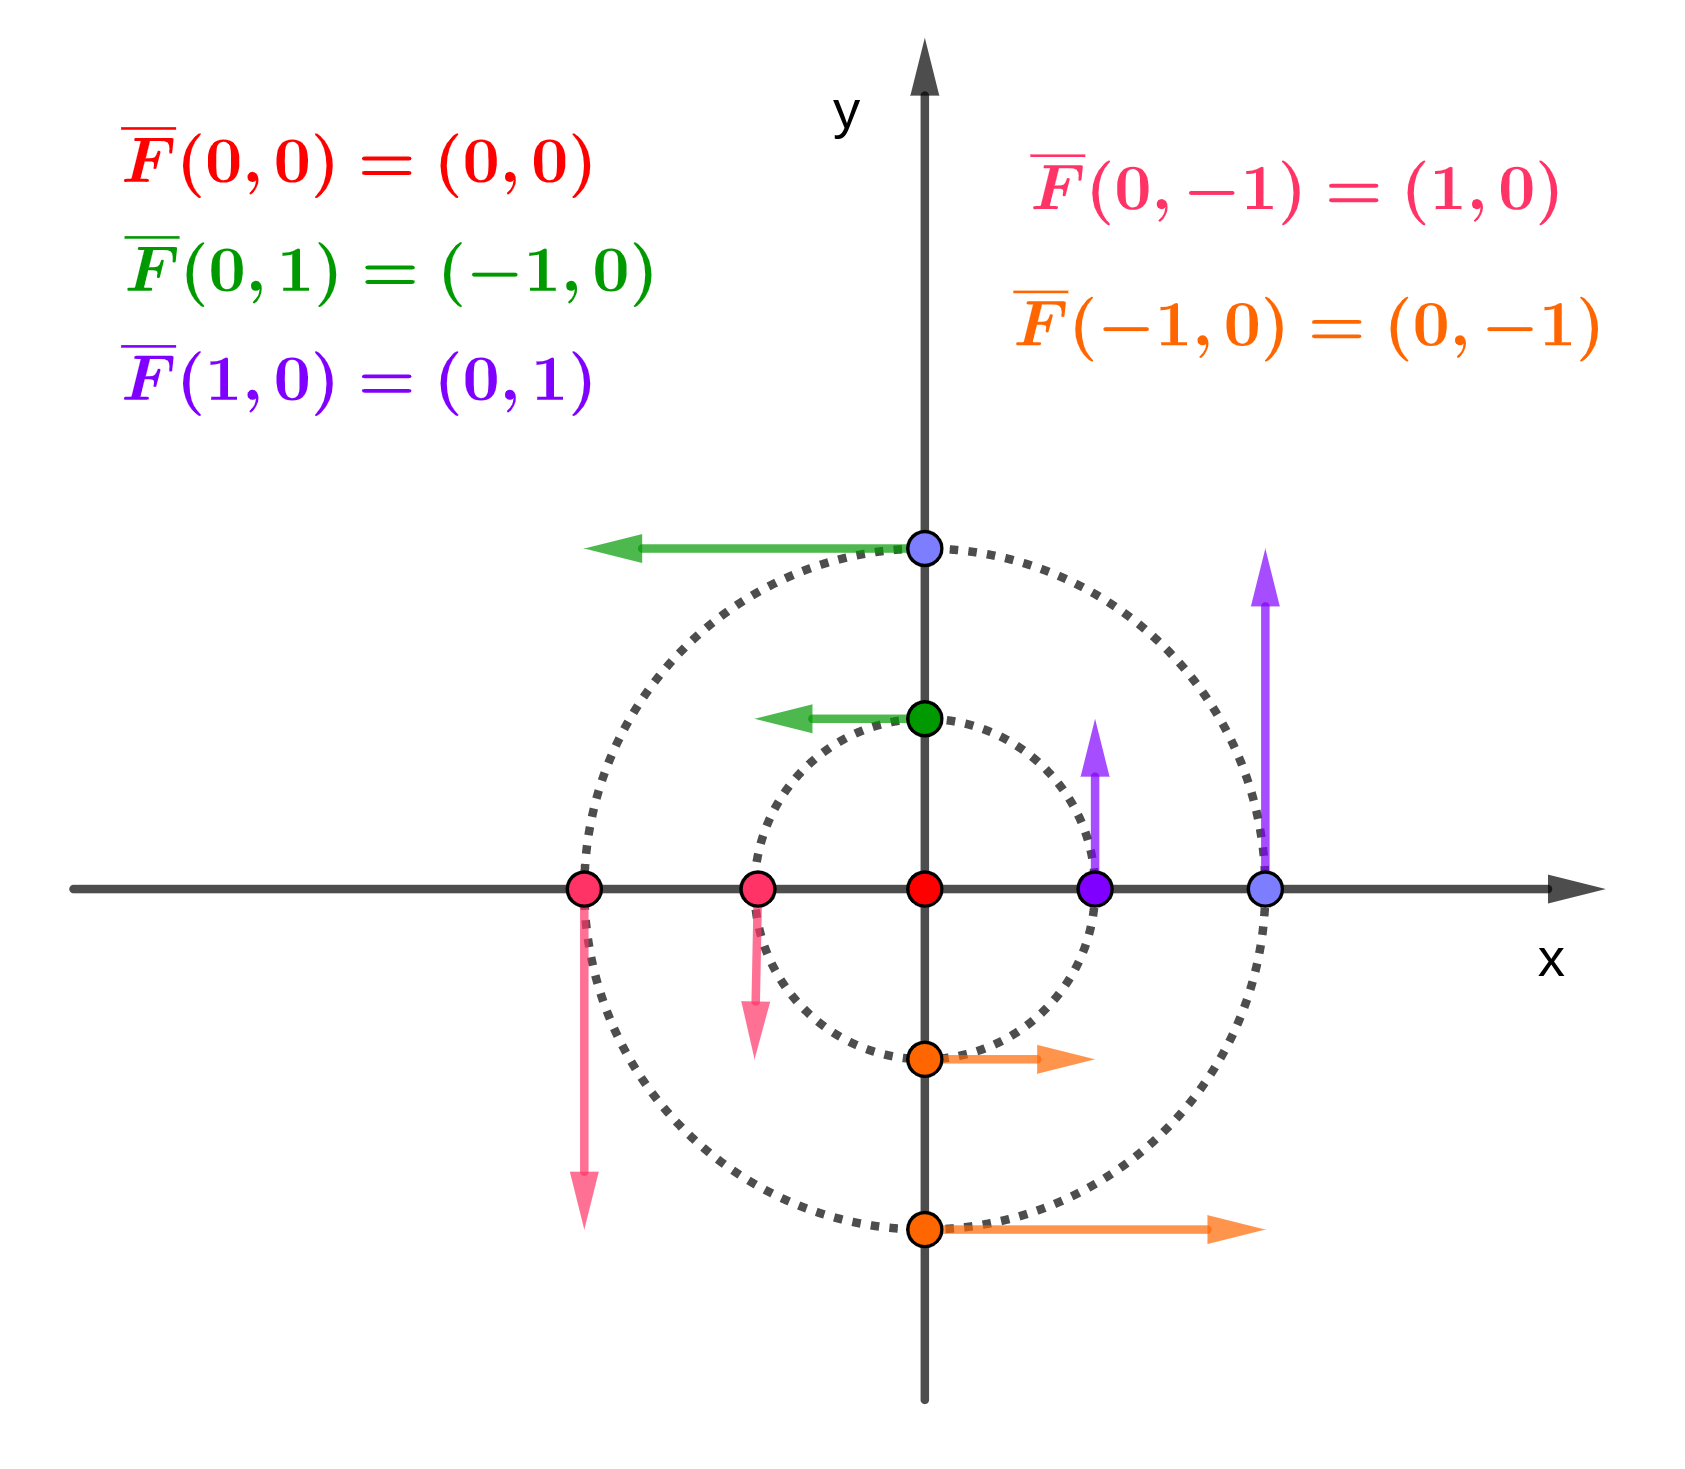
\includegraphics[scale=0.7]{img/edo/lineas_campo.png}
\label{fig:lincamp}
\end{figure}

Si las líneas de campo son curvas cerradas, como en este ejemplo, \textbf{el campo no es conservativo}.

Existen dos métodos para calcular las líneas de campo.

\subsubsection{Resolución vectorial}

Dados el CV (dato) y las líneas de campo (incógnitas):

\begin{align}
& \overline{F}(x,y) = (P(x,y), Q(x,y)) \\
& \overline{g}(t) = (x(t), y(t))
\end{align}

Se plantea la igualdad de la definición para $k = 1$:

\begin{equation}
(P(x(t), y(t), Q(x(t), y(t)) = (x'(t), y'(t))
\end{equation}

De esta igualdad surge un sistema de EDs de 2x2, a partir del cual es posible obtener las ecuaciones paramétricas de $g(t)$.

\subsubsection{Resolución analítica}

Lo primero que se plantea es que, a partir de la definición, los vectores $\overline{F}$ y $\mathop{\overline{dg}}$ son paralelos:

\begin{equation}
\overline{F} \parallel \mathop{\overline{dg}}
\end{equation}

Por otro lado:

\begin{equation}
\mathop{\overline{dg}} = (x'(t), y'(t)) dt = \left( \frac{\mathop{dx}}{\mathop{dt}}, \frac{\mathop{dy}}{\mathop{dt}} \right) \mathop{dt} = (\mathop{dx}, \mathop{dy})
\end{equation}

Ergo:

\begin{align}
(P, Q) \parallel (\mathop{dx}, \mathop{dy}) \Rightarrow \frac{\mathop{dx}}{P} = \frac{\mathop{dy}}{Q} \Rightarrow Q \mathop{dx} = P \mathop{dy} \Rightarrow y' = \frac{Q}{P}
\end{align}

Extensión a $\Bbb R^3$:

\begin{equation}
\frac{\mathop{dx}}{P} = \frac{\mathop{dy}}{Q} = \frac{\mathop{dz}}{R}
\end{equation}

Nótese que en este caso surgen dos igualdades, y por ende un sistema de 2x2.

Otro resultado interesante: si $\overline{F}$ es un CG, las líneas de campo y las equipotenciales son trayectorias ortogonales.

\end{document} 
